\documentclass[a4paper,10pt]{article}
%\usepackage[utf8x]{inputenc}
%\usepackage{czech}
\usepackage[utf8]{inputenc}
\usepackage[czech]{babel}
\usepackage{graphicx}

\title{Zpráva k seminární úloze z předmětu\\ Inteligentní robotika \\ {\small Zpráva č. 2 - Detekce komára v obraze a pohyb v jeho směru}}
\author{Filip Jareš, Lenka Mudrová}
\date{3.4.2011}

\begin{document}

\maketitle

\section{Popis úlohy}

Řešená úloha je inspirována článkem Backyard star wars \cite{clanek}. Pohyblivá kamera sleduje simulovaného komára. Ten je představován černým čtvercem na bílém pozadí monitoru. Pohyb kamery je možné řídit natočením okolo svislé osy (změnou azimutu) a natočením okolo vodorovné osy (změnou elevace). Cílem úlohy je řídit kameru tak, aby sledovala pohyb komára a zdokumentovala jeho „sestřel“ sérií snímků, ve kterých je komár ve středu obrazu z kamery – uprostřed „záměrného kříže“.

\section{Rozbor problému}
\section{Změny specifikace}
\section{Řešení problému}

Rámec programu je tvořen zpětnovazební regulační smyčkou pro řízení polohy kamery. Vstupem regulátoru je nejnovější získaný obrázek z kamery a jeho výstupem je nová poloha kamery. Schematicky je to znázorněno na obrázku \ref{fig:rid_system}.
Před samotným výpočtem nové polohy kamery je vyhodnocen nově získaný obraz. Postup jeho zpracování je znázorněn na obrázku \ref{fig:kamera}.
Nejprve je určena poloha komára v obraze (funkce findMosquitoInImage) v pixelových souřadnicích. Na základě odchylky této polohy od středu obrázku potom funkce mosquitoPxPositionToAzimuthAndElevation počítá odhad úhlů o které je komár vychýlen od optické osy kamery.

\begin{figure}[!htb]
    \centering
     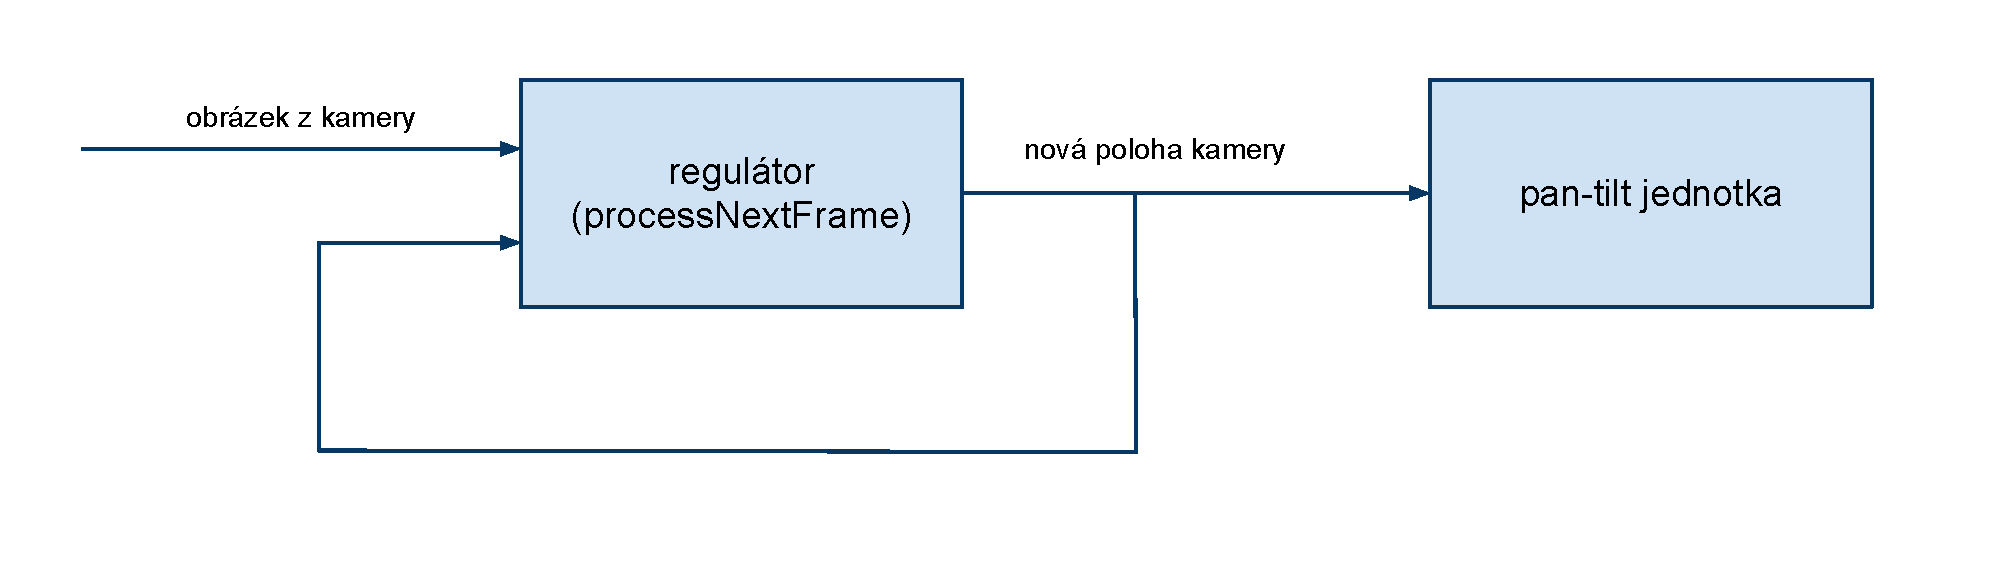
\includegraphics[width=1\columnwidth]{pics/schema_ridiciho_systemu}
     \caption{Schéma řídícího systému\label{fig:rid_system}}
\end{figure}

\begin{figure}[!htb]
    \centering
     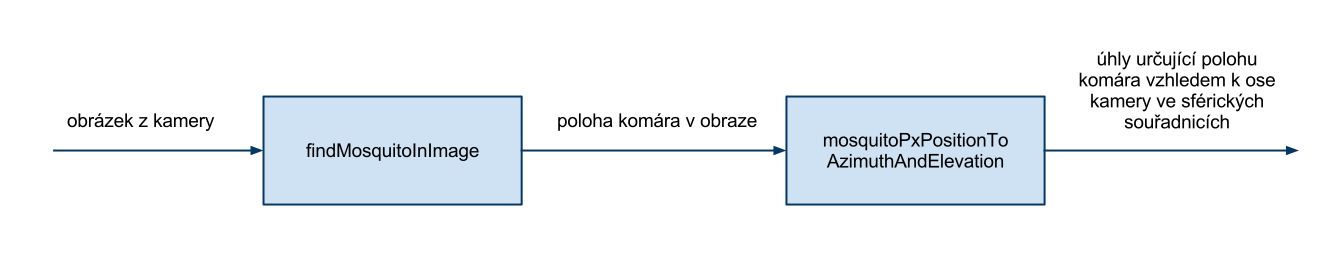
\includegraphics[width=1\columnwidth]{pics/zpracovani_obrazu_z_kamery}
     \caption{Zpracování obrazu z kamery\label{fig:rid_system}}
\end{figure}

\section{Implementace}

Program se spouští hlavní metodou \textit{startMosquitoHunter}:

Po spuštění funce se zinicializuje servo mechanismus tak, aby se kamera nastavila na střed obrazovky, jedná se o startovní konfiguraci, ve která kamera čeká dokud komár nepřilétne do jejího zorného pole. Tento postup je sice pasivní, ale experimenty prokázaly, že oproti aktivímu vyhledávání komára na počátku programu je časově efektivnější. Aktivním vyhledáváním je myšlen algoritmus, kdy kamera sekvenčně snímala pruhy obrazovky a vyhledávala komára.

Dále se zincializuje kamera a s periodou $X? s$ se s využitím callback funkce volá \textit{processNextFrame}, která zahrnuje hlavní chod programu. Perioda je nastavena jako základní testovací, její hodnota se bude ladit do třetí etapy tak, aby byla optimální a omezená pouze parametry kamery a mechanické soustavy. 

\textit{processNextFrame}
Tato funkce vyčte jeden obraz z kamery, upraví ho využitím deBayerizace, Takto upravený obraz předá funkci findMosquitoInImage, která vrátí souřadnice pixelů ve dvou směrech x, y, kde se nachází střed komára. Tyto souřadnice se předají funkci mosquitoPxPositionToAzimuthAndElevation, která vrátí hodnoty azimutu a elevace pro natočení serv. Tyto hodnoty se používají jako referenční a byl implementován jednoduchý P regulátor pro řížení pohybu komára.

?Nezkusíme implementovat PI? Co s windup jevem?
?Oříznutí hodnot na maximální okraj monitoru

findMosquitoInImage

Z barevného obrázku se nejprve vytvoří obrázek šedotónový uložený ve formátu uint8. Po té se naleznou oblasti, ve kterých je podezření na komára na základě znalosti, že komár je tmavý obrazec na světlém pozadí. Tyto oblasti se vyhodnocují na základě histogramu obrázku, hodnoty světlejší než intenzita 200 se zahodí. Tato hodnota byla experimentálně určena, s dostatečnou jistotou oblast komára není světlejší, maximální světlost byla pozorována pod hodnotou 100. Ve zbylé části histogramu se vyhodnotí maximum četností. Práh pro detekci komára je stanoven jako dvojnásobek této hodnoty – dostatečné pokrytí rozložení intenzit kolem maxima. 

Pro oblasti tmavší než daný práh se s využitím funkce regionprops vyhodnotí jejich středy, obsahy a maximální délka osy. Oblasti, jejichž obsah či délka osy přesahuje maximální přípustnou hodnotu pro komára, jsou zahozeny. Tím tedy zůstane oblast odpovídající komárovi, její střed je návratová hodnota této funkce. Výpočetní rychlost algoritmu byla optimalizována, při měření času funkcemi tic, toc byl v průměru naměřen čas 0,08 s.

?zkontrolovat hodnotu

mosquitoPxPositionToAzimuthAndElevation

V této funkci se přepočtou souřadnice v pixelech obrazu na informaci u azimutu a elevaci.

?konkrétnější popis

-----

Detekce komára v obraze z kamery

K získání polohy komára v obrazu z kamery byl použit jednoduchý algoritmus využívající morfologických funkci Matlabovského Image Processing Toolboxu. Byl implementován ve funkci findMosquitoInImage.

Komár zobrazovaný na monitoru pracoviště je představován černým čtvercem na bílém pozadí. Barevná informace je proto zanedbávána a použit je pouze obrázek ve stupních šedi (efektivnější by bylo použít pouze jednu z barevných složek). Tento obrázek je následně oprahován, přičemž jako mez je použita empiricky určená hodnota. V oprahovaném binárním obrázku jsou nalezeny souvislé oblasti. Z nalezených oblastí je vybrána ta, kterou považujeme za komára a je určena poloha jejího středu v pixelových souřadnicích (tj. návratová hodnota funkce findMosquitoInImage).

Při určování oblasti, která odpovídá komárovi, jsou nejprve vyloučeny oblasti, které jsou příliš dlouhé a oblasti, které mají příliš velkou plochu. Ze zbývajících je vybrána ta, která má největší plochu. Plocha oblasti je považována za příliš velkou, je-li větší než přibližně jeden a půl násobek maximální plochy komára v obraze. Oblast je považována za příliš dlouhou, je-li delší, než přibližně dvojnásobek maximální plochy komára.

Z funkcí Image Processing Toolboxu byla použita funkce bwlabel pro nalezení souvislých oblastí a funkce regionprops pro určení délky (vlastnost MajorAxisLength) a plochy (vlastnost Area) těchto oblastí.


\section{Experimentální výsledky}
\section{Diskuze}
\section{Závěr}







\end{document}
